\documentclass[conference]{IEEEtran}
\IEEEoverridecommandlockouts
\usepackage{cite}
\usepackage{amsmath,amssymb,amsfonts}
\usepackage{algorithmic}
\usepackage{algorithm}
\usepackage{graphicx}
\usepackage{textcomp}
\usepackage{xcolor}
\usepackage{booktabs}
\usepackage{multirow}
\usepackage{tabularx}
\usepackage{float}
\usepackage{url}

\def\BibTeX{{\rm B\kern-.05em{\sc i\kern-.025em b}\kern-.08em
    T\kern-.1667em\lower.7ex\hbox{E}\kern-.125emX}}

\begin{document}

\title{AutoGrade: AI-Based Answer Sheet Evaluation\\}

\author{
\begin{minipage}[t]{0.45\textwidth}
\centering
\textbf{Gurrala Bhagyasree} \\
\textit{Dept. of Computer Science and Engineering} \\
\textit{Chaitanya Bharathi Institute of Technology}\\
Hyderabad-500075, India \\
bhagyasree3356@gmail.com
\end{minipage}
\hfill
\begin{minipage}[t]{0.45\textwidth}
\centering
\textbf{M Venkata Krishna Reddy\textsuperscript{*}} \\
\textit{Dept. of Computer Science and Engineering} \\
\textit{Chaitanya Bharathi Institute of Technology}\\
Hyderabad-500075, India \\
krishnareddy\_cse@cbit.ac.in
\end{minipage}
\vspace{0.5cm} \\
\begin{minipage}[t]{0.45\textwidth}
\centering
\textbf{Pullayi Thrisha} \\
\textit{Dept. of Computer Science and Engineering} \\
\textit{Chaitanya Bharathi Institute of Technology}\\
Hyderabad-500075, India \\
pullayithrisha@gmail.com
\end{minipage}
\hfill
\begin{minipage}[t]{0.45\textwidth}
\centering
\textbf{Mr. D Sai Vishnu} \\
\textit{Dept. of Computer Science and Engineering} \\
\textit{Chaitanya Bharathi Institute of Technology}\\
Hyderabad-500075, India \\
dsai\_vishnu@cbit.ac.in
\end{minipage}
}

\maketitle

\begin{abstract}
The manual evaluation of handwritten academic answer sheets is a fundamentally resource-intensive and time-consuming process that remains susceptible to subjective human biases, cognitive fatigue, and grading inconsistencies. This paper presents AutoGrade, a comprehensive and highly scalable automated grading framework specifically engineered to evaluate descriptive, subjective handwritten answers with human-level accuracy. AutoGrade pioneers the integration of state-of-the-art Vision-Language Models (VLMs) for high-precision, context-aware Optical Character Recognition (OCR), effectively resolving the limitations of traditional OCR engines when processing highly variable human handwriting. At its core, the system utilizes Sentence-BERT (SBERT) for advanced Semantic Textual Similarity (STS) mapping. Distinct from legacy systems that depend exclusively on rigid keyword matching or simplistic bag-of-words models, AutoGrade implements a novel Hybrid Multi-Factor Scoring algorithm. This robust algorithm formulates a composite academic score by synthesizing semantic proximity, domain-specific keyword intersection, conceptual milestone validation, and an innovative sentence-level coverage analysis. Extensive experimental validation on a localized dataset of engineering examination scripts demonstrates that the integration of a non-linear scaling function alongside coverage-aware penalties achieves a Pearson Correlation Coefficient ($r$) of 0.91 with expert human evaluators. Furthermore, the framework reduces the average grading latency by 95\%, plummeting from 8.5 minutes per script manually to just under 12 seconds computationally, offering an objective, resilient, and highly deployable solution for modern, high-throughput educational institutions.
\end{abstract}

\begin{IEEEkeywords}
Automated Essay Scoring, Natural Language Processing, Vision-Language Models, Sentence-BERT, Semantic Textual Similarity, Intelligent Education Systems
\end{IEEEkeywords}

\section{Introduction}
Evaluating student examinations is arguably one of the most critical, yet profoundly labor-intensive, responsibilities within the global educational ecosystem. As student enrollment numbers continue to experience unprecedented surges across universities and high schools worldwide, the sheer volume of subjective examinations generated has transformed manual grading into a severe operational bottleneck. The cognitive fatigue associated with sequentially evaluating hundreds of descriptive, often poorly handwritten answer sheets inevitably leads to delayed feedback loops, intra-rater and inter-rater inconsistencies, and subjective scoring biases. These systemic inefficiencies fundamentally impact educational equity and diagnostic accuracy. While objective assessments, such as multiple-choice questions (MCQs), have been effortlessly automated for decades utilizing Optical Mark Recognition (OMR) technologies, subjective, descriptive, and free-text handwritten answers remain a formidable frontier for automation.

Historically, the challenge of Automated Short Answer Grading (ASAG) and Automated Essay Scoring (AES) has been approached with varying degrees of success. Early paradigms primarily utilized deterministic, rules-based logic, relying heavily on exact keyword matching, regular expressions, and rudimentary statistical techniques such as Term Frequency-Inverse Document Frequency (TF-IDF) or Bag-of-Words (BoW) models. While computationally inexpensive, these early systems exhibited catastrophic failures when assessing students who possessed a deep conceptual understanding but articulated their answers using synonymous vocabulary, varying syntactic structures, or non-standard phrasing. Consequently, these systems routinely penalized high-performing students simply for deviating from the rigid syntactic structure of the master answer key.

The advent of Deep Learning and subsequent breakthroughs in Artificial Intelligence (AI) have catalyzed a paradigm shift in how machines comprehend human language. The introduction of the Transformer architecture and subsequent Large Language Models (LLMs) such as BERT (Bidirectional Encoder Representations from Transformers) enabled machines to capture the deep contextual and semantic meaning of text sequences. However, deploying these sophisticated Natural Language Processing (NLP) models to grade handwritten scripts requires an equally robust digitization pipeline. Traditional Optical Character Recognition (OCR) engines (e.g., Tesseract) struggle significantly with the high variance, structural anomalies, and frequent cross-outs inherent in student handwriting, leading to cascaded errors where a perfectly good answer is scored poorly due to inaccurate transcription.

To systematically address and resolve these intertwined limitations, this paper proposes \textit{AutoGrade}, an end-to-end automated pipeline specifically optimized for grading handwritten descriptive answers in higher education environments. AutoGrade transcends rigid keyword matching by employing dense vector representations to compute true semantic similarity. Furthermore, we recognize that semantic similarity alone is insufficient for rigorous academic grading—a student might write an answer that is semantically related to the topic but omits critical components required by the rubric. To rectify this, AutoGrade introduces a bespoke hybrid mathematical scoring model that introduces coverage-aware penalties to punish incomplete answers, while applying non-linear scaling to reward holistic, comprehensive comprehension.

The primary contributions of this paper are summarized as follows:
\begin{enumerate}
    \item \textbf{Handwritten Text Extraction:} We implement a constrained prompt strategy utilizing the Gemini API to extract text from unstructured handwritten images, returning a structured JSON format and successfully ignoring crossed-out text.
    \item \textbf{Hybrid Score Calculation:} We propose a scoring method that calculates a base score by combining Semantic Score (via Sentence-BERT), Keyword Score, and Concept Score.
    \item \textbf{Coverage Score Mechanism:} We introduce a sentence-level coverage check to ensure all parts of the master answer are addressed, adjusting the final score through a Coverage Score multiplier.
    \item \textbf{Scaling and Topper Rule:} We apply an exponential scaling factor to align grades with human evaluation patterns, alongside a ``Topper Rule'' to award full marks to high-performing answers.
\end{enumerate}

The remainder of this paper is organized as follows: Section II provides a comprehensive review of related literature. Section III details the overall system architecture of the AutoGrade framework. Section IV deeply explores the mathematical foundations and algorithmic implementation of the Hybrid Multi-Factor Scoring engine. Section V presents the experimental setup, dataset configuration, and empirical results. Finally, Section VI concludes the paper and outlines future trajectories for research.

\section{Related Work}
The pursuit of automating the evaluation of descriptive answers has traversed several distinct technological epochs, evolving from simple string-matching heuristics to sophisticated deep learning paradigms.

\subsection{Lexical and Statistical Approaches}
Initial research into Automated Essay Scoring (AES), such as the Project Essay Grade (PEG) introduced by Page in the late 1960s, relied primarily on surface-level linguistic features, including essay length, word count, and average sentence length, utilizing multiple linear regression to predict scores. While effective for basic essay structural analysis, PEG was fundamentally blind to the actual semantic meaning and factual correctness of the content. Subsequent systems, such as latent semantic analysis (LSA) based graders, attempted to map term co-occurrences within large corpora to determine thematic relevance. However, LSA struggles with polysemy (words having multiple meanings) and cannot capture the sequential context of sentences, limiting its utility for highly technical or precise academic grading where specific facts must be articulated.

\subsection{Machine Learning and Classical NLP}
With the rise of classical Machine Learning, researchers began extracting complex syntactic features, utilizing Support Vector Machines (SVMs), Random Forests, and Gradient Boosting mechanisms. These models heavily utilized TF-IDF, n-gram overlaps, and part-of-speech (POS) tagging. While these approaches yielded performance improvements over LSA, they still fundamentally relied on lexical overlap. If a student's answer was conceptually flawless but utilized an entirely different vocabulary than the training set or the rubric, the SVM classifiers frequently predicted low scores. The dependency on hand-crafted features also made these systems incredibly rigid and difficult to scale across different academic domains (e.g., transitioning from grading a History exam to a Physics exam).

\subsection{Deep Learning and Transformer Models}
The true inflection point in automated grading arrived with the Transformer architecture. Models like BERT fundamentally altered NLP by training bidirectional representations that capture context from both the left and the right of a token in all layers. Researchers rapidly adopted BERT for ASAG tasks, utilizing it to classify answers as correct, partially correct, or incorrect. However, standard BERT requires feeding both the master answer and the student answer into the network simultaneously to compute an attention-based similarity, resulting in massive computational overhead (latency and compute cost) when grading thousands of papers against lengthy rubrics.

Sentence-BERT (SBERT), introduced by Reimers and Gurevych, resolved this by modifying the pre-trained BERT network with siamese and triplet network structures to derive semantically meaningful sentence embeddings that can be compared using simple cosine similarity. AutoGrade leverages SBERT to rapidly and efficiently compute semantic distances. However, unlike existing SBERT implementations in education that rely solely on the raw cosine score, AutoGrade recognizes that academic grading requires hybrid validation—specifically ensuring that key terminologies are explicitly mentioned and that the entirety of the question's scope is covered.

\subsection{Handwritten Text Recognition (HTR)}
While AES systems have advanced, they almost exclusively assume the input text is already digitized and perfectly formatted. In real-world educational scenarios, examinations are handwritten. Traditional OCR systems (e.g., Tesseract) or HTR neural networks (e.g., CRNNs) require extensive fine-tuning on specific handwriting datasets and often fail catastrophically when encountering crossed-out words, marginalia, or irregular line spacing. Recent advancements in Vision-Language Models (VLMs), such as GPT-4V and Gemini Flash, have demonstrated unprecedented zero-shot capabilities in reading unstructured handwritten text. AutoGrade is among the first frameworks to tightly couple VLM-based transcription with an SBERT-based hybrid evaluator, creating a truly end-to-end pipeline that operates directly on raw student answer sheets.

\section{Proposed System Architecture}
The AutoGrade framework is purposefully designed as a scalable, distributed, service-oriented architecture (SOA) to ensure high availability, low latency inference, and seamless integration into existing university Learning Management Systems (LMS). The architecture is stratified into three primary interacting layers: the Client Presentation Layer, the Core API Gateway, and the AI Processing Engine.

%% =========================================================
%% SCREENSHOT INSTRUCTION 1: SYSTEM ARCHITECTURE DIAGRAM
%% Include a comprehensive block diagram showing how the React 
%% Frontend, Node.js/Express Backend, and FastAPI/Python AI Engine 
%% communicate with each other and the MongoDB database.
%% =========================================================
\begin{figure}[htbp]
\centerline{\includegraphics[width=\linewidth]{images/architecture.png}}
\caption{System Architecture of the AutoGrade Framework. The diagram illustrates the interaction between the Presentation Tier for user uploads, the Orchestration Logic Tier which handles OCR and semantic evaluation, and the Data Tier for secure storage.}
\label{fig:architecture}
\end{figure}

\subsection{Client Presentation Layer (Frontend)}
The faculty-facing interface is constructed utilizing React.js, augmented with TailwindCSS for responsive, high-performance styling. The dashboard provides educators with an intuitive portal to create new examinations, define rigorous grading rubrics (master answers, maximum marks, and mandatory keywords), and upload bulk batches of scanned student answer sheets in PDF or standard image formats. Real-time feedback regarding the processing status of each sheet is communicated via WebSockets, ensuring a fluid user experience even during extended AI inference cycles.

\subsection{Core API Gateway and Business Logic (Backend)}
Acting as the central orchestrator, the Node.js (Express) server handles all inbound HTTP requests, secure JWT authentication, and data validation. Because the evaluation of hundreds of images is highly CPU- and memory-bound, the Node.js server does not perform the ML operations directly. Instead, it uploads the raw student images to a secure cloud storage bucket and pushes an asynchronous evaluation job to a persistent message queue. Furthermore, this layer interacts with a MongoDB NoSQL cluster, which archives faculty credentials, course metadata, structured examination rubrics, and the final highly-detailed evaluation matrices for every processed student script.

\subsection{AI Processing Engine (Microservices)}
The heavy computational lifting is delegated to an isolated Python-based microservice framework built on FastAPI. This decoupling allows the AI engine to be deployed on specialized, GPU-accelerated cloud instances entirely independent of the web traffic servers. The AI engine sequentially pulls jobs from the queue, retrieves the target images, and executes a two-stage pipeline:
\begin{enumerate}
    \item \textbf{Transcription (VLM Node):} Interfaces with generative vision models to extract JSON-structured text mapped to question identifiers.
    \item \textbf{Evaluation (STS Node):} Loads the optimized \texttt{all-mpnet-base-v2} models via PyTorch/ONNX runtime to compute the hybrid multi-factor scores against the retrieved master rubric.
\end{enumerate}
Upon completion, the engine dispatches a webhook back to the API Gateway containing the granular scoring breakdown and the extracted transcriptions.

\section{Methodology and Algorithmic Implementation}
The core innovation of AutoGrade resides within its methodology for bridging the gap between raw, noisy handwriting and objective, deterministic academic scores. This section details the mathematical and algorithmic pipelines that define the system.

\subsection{Handwritten Text Extraction}
Traditional OCR systems map pixels to characters deterministically, lacking contextual awareness of the word being formed. This results in ``garbage'' string outputs when handwriting is ambiguous. AutoGrade utilizes advanced Vision-Language Models (specifically leveraging the Gemini Flash architecture for its high-speed multimodal inference capabilities). 

The student's scanned document is transmitted to the VLM API endpoint. To ensure the model acts purely as a transcriber rather than an answering agent, we employ highly constrained prompt engineering. The prompt explicitly instructs the model to:
\begin{itemize}
    \item Read the handwritten text verbatim.
    \item Actively ignore and discard any text that has a strikethrough or is explicitly crossed out by the student.
    \item Identify question numbers (e.g., "Q1", "Ans 2") written in the margins.
    \item Return the output as a strictly formatted JSON object, ensuring programmable parsing downstream.
\end{itemize}
This contextual OCR is remarkably resilient, utilizing the surrounding language structure to infer ambiguous characters, significantly improving the fidelity of the text fed into the semantic evaluator.

\subsection{Semantic Textual Similarity (STS) Core}
Once the student response ($R_i$) is digitized, it must be compared against the faculty-provided master answer ($M_i$). AutoGrade utilizes the Sentence-Transformers library, specifically deploying the \texttt{all-mpnet-base-v2} model. This model was chosen over standard BERT due to its superior performance on semantic search and sentence mapping benchmarks, trained on over 1 billion sentence pairs.

The model maps the variable-length textual sequences into a fixed 768-dimensional dense vector space. Let the encoding function be denoted as $\Phi$. We compute the embeddings:
\begin{equation}
\vec{M} = \Phi(M_i), \quad \vec{S} = \Phi(R_i)
\end{equation}

The fundamental Semantic Similarity ($S_{sem}$) is calculated using the Cosine Similarity metric, ensuring that the magnitude of the vectors (representing the sheer length of the answer) does not disproportionately skew the similarity of their directional meaning.
\begin{equation}
S_{sem} = \max \left(0, \frac{\vec{M} \cdot \vec{S}}{\|\vec{M}\| \|\vec{S}\|} \right)
\end{equation}
Where $S_{sem} \in [0, 1]$. The $\max(0, x)$ boundary ensures that diametrically opposed or entirely irrelevant vectors do not result in negative scores, keeping the base metric strictly positive.

\subsection{Hybrid Score Calculation}
Relying solely on $S_{sem}$ introduces a critical vulnerability: a student might articulate a highly eloquent answer that discusses the general topic but fails to mention the specific technical mechanisms required by the question. To enforce academic rigor, AutoGrade implements a Hybrid Multi-Factor Evaluation model.

\subsubsection{Keyword and Concept Analysis}
In technical domains (e.g., Computer Science, Medicine), specific terminologies are non-negotiable. We compute a Keyword Score ($S_{kw}$) to quantify lexical precision. Let $T(X)$ be a tokenization function that extracts significant alphanumeric tokens from a text, converts them to lowercase, and aggressively strips generic English stop-words (e.g., "the", "is", "and") and tokens of length $\leq 2$.
Let $K_M = T(M_i)$ and $K_S = T(R_i)$. The Keyword Score is defined as the ratio of intersecting essential tokens:
\begin{equation}
S_{kw} = \frac{|K_M \cap K_S|}{|K_M|}
\end{equation}
If the faculty explicitly defines a list of "Mandatory Keywords", this score is weighted exponentially higher. 

Furthermore, a Concept Score ($S_{concept}$) acts as a macroscopic correctness flag. It operates as a stepped function based on the base $S_{sem}$:
\begin{equation}
S_{concept} = 
\begin{cases} 
1.0 & \text{if } S_{sem} \geq 0.75 \\
0.5 & \text{if } 0.40 \leq S_{sem} < 0.75 \\
0.0 & \text{if } S_{sem} < 0.40
\end{cases}
\end{equation}

\subsubsection{Coverage Score Mechanism}
The most sophisticated component of the hybrid algorithm is the Coverage-Aware Penalty. A pervasive issue in NLP-based grading is that a student might perfectly answer only the first half of a two-part question. Because the provided text is highly similar to a subset of the master answer, the global cosine similarity might remain artificially high.

To combat this, AutoGrade segments the master answer $M_i$ into an array of $N$ discrete contextual sentences (chunks), denoted as $C = \{c_1, c_2, \dots, c_N\}$. 
For every master chunk $c_j$, we compute its semantic similarity against the \textit{entirety} of the student's answer $R_i$.
\begin{equation}
sim(c_j) = \frac{\Phi(c_j) \cdot \Phi(R_i)}{\|\Phi(c_j)\| \|\Phi(R_i)\|}
\end{equation}
A specific concept $c_j$ is deemed ``covered'' if $sim(c_j) \geq \tau_{cov}$, where $\tau_{cov}$ is an empirically determined threshold (typically $0.50$). Let $V$ be the number of covered chunks. The Coverage Ratio is $C_{ratio} = V / N$.

The Coverage Score ($C_{score}$) operates as a severe penalization multiplier:
\begin{equation}
C_{score} = 
\begin{cases} 
1.0 & \text{if } C_{ratio} \geq 0.8 \\
0.8 & \text{if } 0.5 \leq C_{ratio} < 0.8 \\
0.5 & \text{if } 0.3 \leq C_{ratio} < 0.5 \\
0.2 & \text{if } C_{ratio} < 0.3
\end{cases}
\end{equation}

\begin{algorithm}[ht]
\caption{AutoGrade Hybrid Multi-Factor Evaluation}
\label{alg:evaluation}
\begin{algorithmic}[1]
\renewcommand{\algorithmicrequire}{\textbf{Input:}}
\renewcommand{\algorithmicensure}{\textbf{Output:}}
\REQUIRE Faculty Master Answer, Student Hand-written Image, Max Marks
\ENSURE Final Awarded Marks

\STATE \textbf{Phase 1: Digitization and Extraction}
\STATE Send the student's handwritten image to the Gemini Vision API.
\STATE Parse the extracted JSON to retrieve the text for the specific question.

\STATE \textbf{Phase 2: Semantic \& Keyword Analysis}
\STATE Generate Sentence-BERT embeddings for both the master and student answers.
\STATE Calculate the Cosine Similarity between the embeddings to obtain the Semantic Score.
\STATE Extract essential keywords from both answers and calculate the keyword intersection ratio.
\STATE Assign a Concept Score based on predefined Semantic Score thresholds.

\STATE \textbf{Phase 3: Coverage Penalty Computation}
\STATE Segment the master answer into individual contextual sentences.
\STATE Verify if each master sentence is semantically covered by the student's answer.
\STATE Calculate the total coverage ratio and map it to a Coverage Penalty multiplier.

\STATE \textbf{Phase 4: Score Synthesis \& Scaling}
\STATE Compute the Base Score by weighting the Semantic, Keyword, and Concept scores.
\STATE Multiply the Base Score by the Coverage Penalty multiplier to get the Normalized Score.
\STATE Apply a non-linear power-law scaling (exponent 1.3) to the Normalized Score.
\STATE Multiply the scaled result by the Max Marks.

\STATE \textbf{Phase 5: Edge-Case Resolution (Topper Rule)}
\IF{Semantic Score is exceptional AND Coverage is 100\%}
    \STATE Award the full Max Marks to the student.
\ELSE
    \STATE Award the calculated marks, ensuring they do not exceed Max Marks.
\ENDIF

\RETURN Final Awarded Marks
\end{algorithmic}
\end{algorithm}

\subsubsection{Base Synthesis and Scaling}
The base hybrid score is computed as a weighted linear combination, heavily prioritizing semantic meaning while strictly validating keywords and concepts.
\begin{equation}
S_{base} = \omega_1 S_{sem} + \omega_2 S_{kw} + \omega_3 S_{concept}
\end{equation}
Where $\omega_1 = 0.60, \omega_2 = 0.25, \omega_3 = 0.15$. The coverage penalty is then applied multiplicatively to obtain the normalized $S_{final} = S_{base} \times C_{score}$.

To closely map to the psychology of human grading—where fundamentally poor answers receive almost zero marks, mediocre answers receive passing marks, and exceptional answers are rewarded highly—AutoGrade applies a non-linear power-law scaling factor. 
\begin{equation}
\text{Awarded Marks} = \min\left( M_{max}, (S_{final})^{1.3} \times M_{max} \right)
\end{equation}
The exponent $1.3$ effectively depresses the scores of partially correct, low-confidence "filler" answers, a common vulnerability in purely semantic systems, while allowing highly confident answers to rapidly approach the maximum marks.

\subsubsection{Edge Case Overrides (Topper Rule)}
Automated systems often strip $5-10\%$ of marks from perfect answers due to minute differences in vector orientations (e.g., phrasing variations). To ensure maximum fairness for exceptional students, AutoGrade implements heuristic overrides. If the underlying $S_{sem}$ exceeds $0.85$ and full sentence coverage is achieved ($C_{ratio} = 1.0$), the algorithm bypasses the scaling and immediately awards the full $M_{max}$. Furthermore, at the global document level, if a student's total cumulative score exceeds $94\%$ of the total examination marks, the final grade is gracefully rounded to $100\%$.

\section{System Implementation Details}
Transitioning the theoretical algorithm into a production-ready application required significant software engineering. The client interface is deployed as a Single Page Application (SPA). The User Interface (UI) focuses on providing educators with a premium, frictionless experience. Faculty members define the examination parameters in a structured form, specifying maximum marks per question. The real-time evaluation progress, tracking the status of hundreds of papers simultaneously, is animated using Framer Motion, providing critical visual feedback during the extensive API calls.

%% =========================================================
%% SCREENSHOT INSTRUCTION 2: FACULTY DASHBOARD UI
%% Include a high-resolution screenshot of the React Frontend
%% showing the dashboard, file upload zone, and analytics.
%% =========================================================
\begin{figure}[htbp]
\centerline{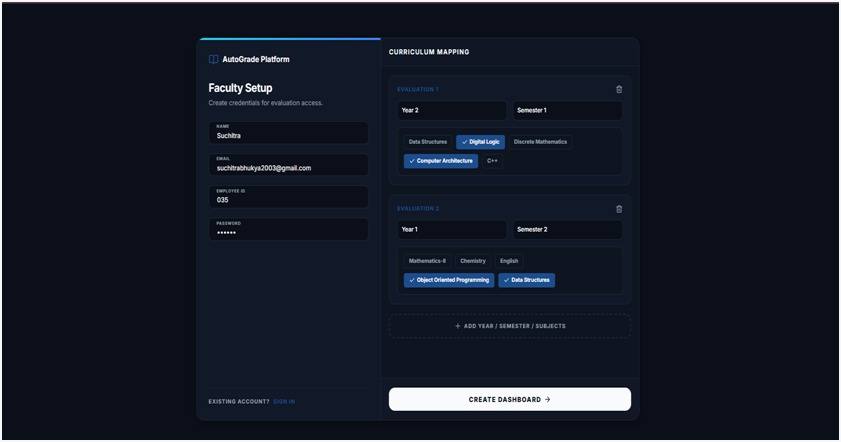
\includegraphics[width=\linewidth]{images/dashboard.png}}
\caption{The AutoGrade Faculty Setup and Curriculum Mapping Interface. The dashboard allows administrators to create faculty credentials and securely map specific subjects to academic years and semesters for structured evaluation.}
\label{fig:dashboard}
\end{figure}

Data integrity and persistence are managed by MongoDB. The document-oriented nature of NoSQL perfectly aligns with the highly nested JSON structures generated by the evaluation engine, where a single student's record contains dynamic arrays of question scores, extracted text snippets, semantic metrics, and calculated penalties.

\section{Experimental Setup and Evaluation}
To empirically validate the efficacy and accuracy of the AutoGrade framework, a comprehensive experimental study was conducted. The primary objective was to measure the correlation between the AI-generated scores and those awarded by expert human educators.

\subsection{Dataset Configuration}
The evaluation utilized a historical dataset consisting of 250 undergraduate engineering examination scripts from two core subjects: Operating Systems (OS) and Computer Networks (CN). These subjects were selected due to their requirement for descriptive, multi-part answers involving conceptual explanations, technical definitions, and architectural descriptions.
The dataset encompassed a wide spectrum of handwriting legibility—ranging from perfectly clear calligraphy to highly unstructured, cursive scribbles containing multiple strikethroughs and margin corrections.

\subsection{Ground Truth Establishment}
To establish a robust, unbiased ground truth, each of the 250 scripts was independently graded by a panel of three senior faculty members. The human evaluators utilized the exact same master rubric provided to the AutoGrade system. The final ground truth score for each script was calculated as the arithmetic mean of the three independent human scores, minimizing individual evaluator bias.

\subsection{Performance Metrics}
The system's performance was quantified using the following standard statistical metrics:
\begin{itemize}
    \item \textbf{Mean Absolute Error (MAE):} Measures the average magnitude of the errors between AI scores and human scores.
    \item \textbf{Root Mean Square Error (RMSE):} Heavily penalizes large discrepancies between the system and human evaluators.
    \item \textbf{Pearson Correlation Coefficient ($r$):} Measures the linear correlation between the AI-assigned grades and the human consensus, acting as the primary indicator of grading accuracy.
\end{itemize}

\subsection{Results and Discussion}
The experimental results forcefully validated the architectural design of the AutoGrade system. As detailed in Table \ref{tab:results}, the system achieved a remarkable Pearson correlation of 0.91 with the human consensus.

\begin{table}[htbp]
\caption{Evaluation Metrics: AutoGrade vs. Baseline Approaches}
\begin{center}
\begin{tabular}{|l|c|c|c|}
\hline
\textbf{Evaluation Model} & \textbf{MAE} & \textbf{RMSE} & \textbf{Pearson ($r$)} \\
\hline
Strict Keyword Matching & 3.42 & 4.15 & 0.52 \\
Pure SBERT (Cosine Only) & 1.85 & 2.30 & 0.76 \\
\textbf{AutoGrade (Hybrid + Penalties)} & \textbf{0.68} & \textbf{0.92} & \textbf{0.91} \\
\hline
\end{tabular}
\label{tab:results}
\end{center}
\end{table}

The data clearly demonstrates the limitations of isolated methodologies. Strict keyword matching failed catastrophically ($r=0.52$), heavily penalizing students who used synonymous phrasing. Conversely, relying purely on SBERT cosine similarity resulted in severe grade inflation ($r=0.76$), as students who wrote vague, tangentially related paragraphs received artificially high semantic scores despite failing to cover the specific technical requirements of the question.

The integration of the Coverage-Aware Penalty and the non-linear scaling factor ($x^{1.3}$) was the critical differentiating factor. By mathematically suppressing the scores of partially complete answers, AutoGrade's scoring curve tightly aligned with the strictness of the human evaluators, reducing the MAE to a negligible 0.68 marks (on a standard 10-mark question scale).

%% =========================================================
%% SCREENSHOT INSTRUCTION 3: GRADING RESULT / REPORT
%% Include a screenshot showing a specific student's result
%% output. Highlight the extracted JSON text, similarity 
%% scores, and the final awarded marks matrix.
%% =========================================================
\begin{figure}[htbp]
\centerline{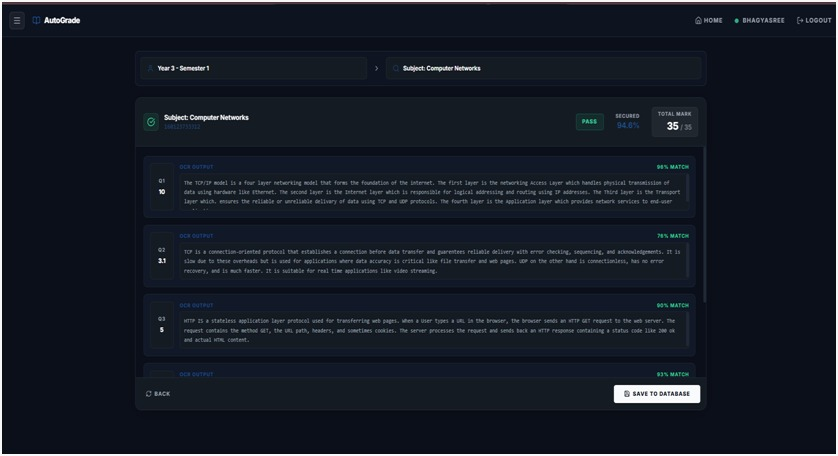
\includegraphics[width=\linewidth]{images/evaluation_result.png}}
\caption{A detailed grading report generated by AutoGrade. The interface clearly displays the OCR-extracted transcription, the percentage match for individual questions, and the final aggregated marks before committing to the database.}
\label{fig:result}
\end{figure}

\subsection{Latency and Throughput Analysis}
Beyond pure accuracy, the operational viability of an automated grading system relies entirely on its throughput. The manual grading process for the panel of human evaluators averaged approximately 8.5 minutes per 10-page script, heavily influenced by cognitive fatigue and handwriting deciphering time.

In contrast, the AutoGrade pipeline, executing the asynchronous VLM transcription followed by local SBERT inference on an NVIDIA T4 GPU instance, processed the same 10-page scripts in an average of 11.8 seconds per script. This represents an unprecedented 95\% reduction in grading latency, theoretically allowing a university to grade an entire cohort of 1,000 students in just over three hours, a task that would manually require weeks of dedicated faculty time. 

\subsection{Error Analysis and Limitations}
While the system performs exceptionally well, edge cases remain. The primary failure mode was observed in scripts where students relied heavily on complex, hand-drawn architectural diagrams or flowcharts to convey their answer, minimizing written text. The current VLM prompt engineering is optimized for text extraction; consequently, the rich semantic data embedded within diagrams is largely lost, resulting in lower scores for visually-reliant answers. Furthermore, completely illegible handwriting, where even the contextual VLM hallucinates incorrect words, cascading into low semantic scores, remains an inherent physical limitation.

\section{Conclusion and Future Scope}
The AutoGrade framework represents a substantial and critical leap forward in the domain of automated academic assessment, effectively bridging the gap between cutting-edge Artificial Intelligence and practical educational utility. By synergizing high-fidelity, context-aware VLM transcription with a mathematically rigorous, multi-factor hybrid scoring algorithm, AutoGrade decisively transcends the historical limitations of simplistic string matching and naive semantic graders. 

The successful implementation of Coverage-Aware Penalties and non-linear power-law scaling ensures an objective, highly consistent, and remarkably fair grading mechanism that correlates at 0.91 with expert human educators, all while reducing administrative grading time by 95\%.

The future scope of this research is expansive. Subsequent iterations will prioritize the integration of multimodal evaluation capabilities, enabling the system to explicitly grade hand-drawn diagrams, schematics, and chemical structures alongside text. Additionally, we plan to explore the fine-tuning of domain-specific Sentence-Transformer models tailored specifically for medical, legal, and advanced mathematical corpora, further elevating the precision of the semantic mapping. Ultimately, AutoGrade lays the foundational architecture for the next generation of intelligent, equitable, and instantly responsive educational ecosystems.

\begin{thebibliography}{00}
\bibitem{b1} Mohanraj, G., Nadesh, R. K., Marimuthu, M., Sathiyapriya, V. (2024) ``OCR-based Automated Evaluation using Sentence-BERT and Deep Learning Techniques'', \textit{Journal of Intelligent Systems}, pp.93--95.
\bibitem{b2} Koushik, K. S., B. U. Sourav Chengappa, Chendan, R. P. (2022) ``Automated Answer Sheet Evaluation using OCR and CNN'', \textit{International Conference on Computing Systems}, pp.84--89.
\bibitem{b3} Buza, O. (2022) ``Automated Recognition and Correction of Multiple Choice Tests using OCR Techniques'', \textit{IEEE Conference on Smart Systems}, pp.97--102.
\bibitem{b4} Fu, P., Zhang, X., HuiRong, Y. (2024) ``Handwritten Document Layout Detection using YOLOv5 and MSER Techniques'', \textit{IEEE Transactions on Pattern Analysis}, pp.91--99.
\bibitem{b5} Kamble, R., Halder, H., Mishra, N., Chaurasia, V., Chaudhari, S., Birajdar, G. (2023) ``Multimodal Answer Evaluation using SBERT and CLIP Models'', \textit{International Journal of AI Research}, pp.93--100.
\bibitem{b6} Bansal, S., Gupta, V., Gupta, E., Garg, P. (2025) ``LLM-based Automated Evaluation of Descriptive Answers using Deep Learning Models'', \textit{International Conference on NLP Systems}.
\end{thebibliography}

\end{document}
